\begin{frame}[ctb!]
  \frametitle{Development : From GENIUS to Cyclus}
  The predecessor of Cyclus was a simulator named GENIUSv2 \cite{oliver_geniusv2:_2009}
  \begin{itemize}
    \item also written in C++
    \item similar structures (regions - institutions - facilities)
    \item designed to overcome other simulator's difficulties
    \item not designed to proliferate a community
  \end{itemize}
\end{frame}

\begin{frame}[ctb!]
  \frametitle{Development : Developer Environment}
  Cyclus is designed to accommodate any kind of user or developer by
  allowing flexible participation \cite{huff_prelim_2011}
  \begin{figure}[htbp!]
    \begin{center}
      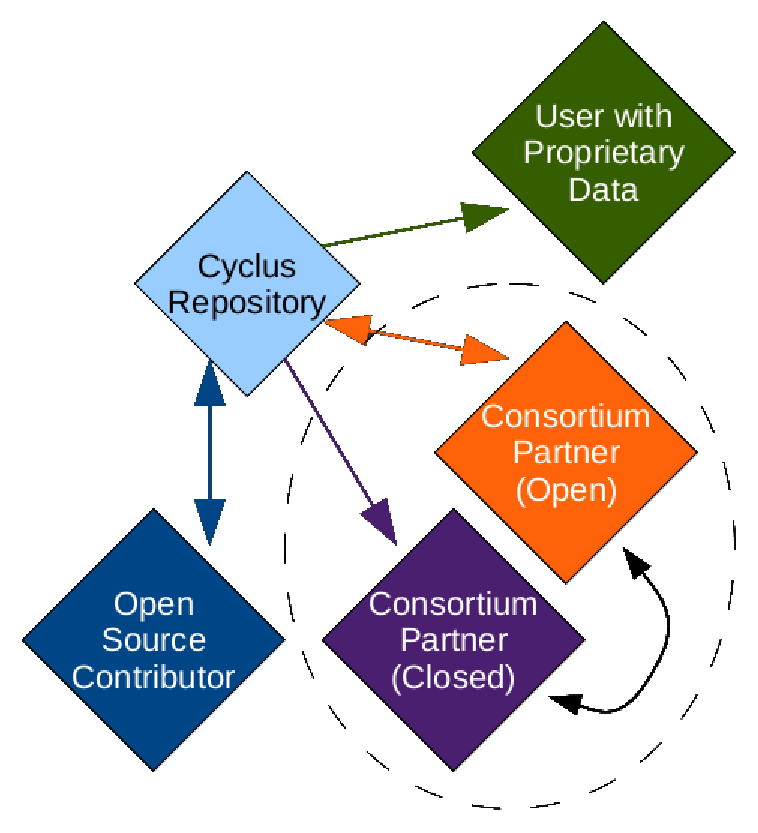
\includegraphics[height=4cm]{community.eps}
    \end{center}
    \caption{The Cyclus Participation Paradigm} 
    \label{fig:community}
  \end{figure}
\end{frame}

\begin{frame}[ctb!]
  \frametitle{Development : Code Repository}
  The Cyclus code repository is publicly available on GitHub.

  \vspace{0.2cm}

  General information can be found at cyclus.github.com.
  \begin{figure}[htbp!]
    \begin{center}
      \includegraphics[height=4cm]{cyclus-github.ps}
    \end{center}
    \caption{The Cyclus Github Landing Page} 
    \label{fig:cyclus-github}
  \end{figure}
\end{frame}

\begin{frame}[ctb!]
  \frametitle{Development : Code Repository}
  The Cyclus code repository is publicly available on GitHub.

  \vspace{0.2cm}

  The Cyclus source code can be found at github.com/cyclus/core.
  \begin{figure}[htbp!]
    \begin{center}
      \includegraphics[height=4cm]{github-core.ps}
    \end{center}
    \caption{The Cyclus Source Code Repository} 
    \label{fig:github-core}
  \end{figure}
\end{frame}

\begin{frame}[ctb!]
  \frametitle{Development : Model Modularity}
  Combined with the availability of the Cyclus engine source code,
  modularity of models in Cyclus plays a pivotal role in reducing its
  barriers to entry.

  \vspace{0.2cm}
  
  The Cyclus engine defines a Model's API, to which all models must
  conform. This allows models of each archetype to be interchangeable.
  \begin{figure}[htbp!]
    \begin{center}
      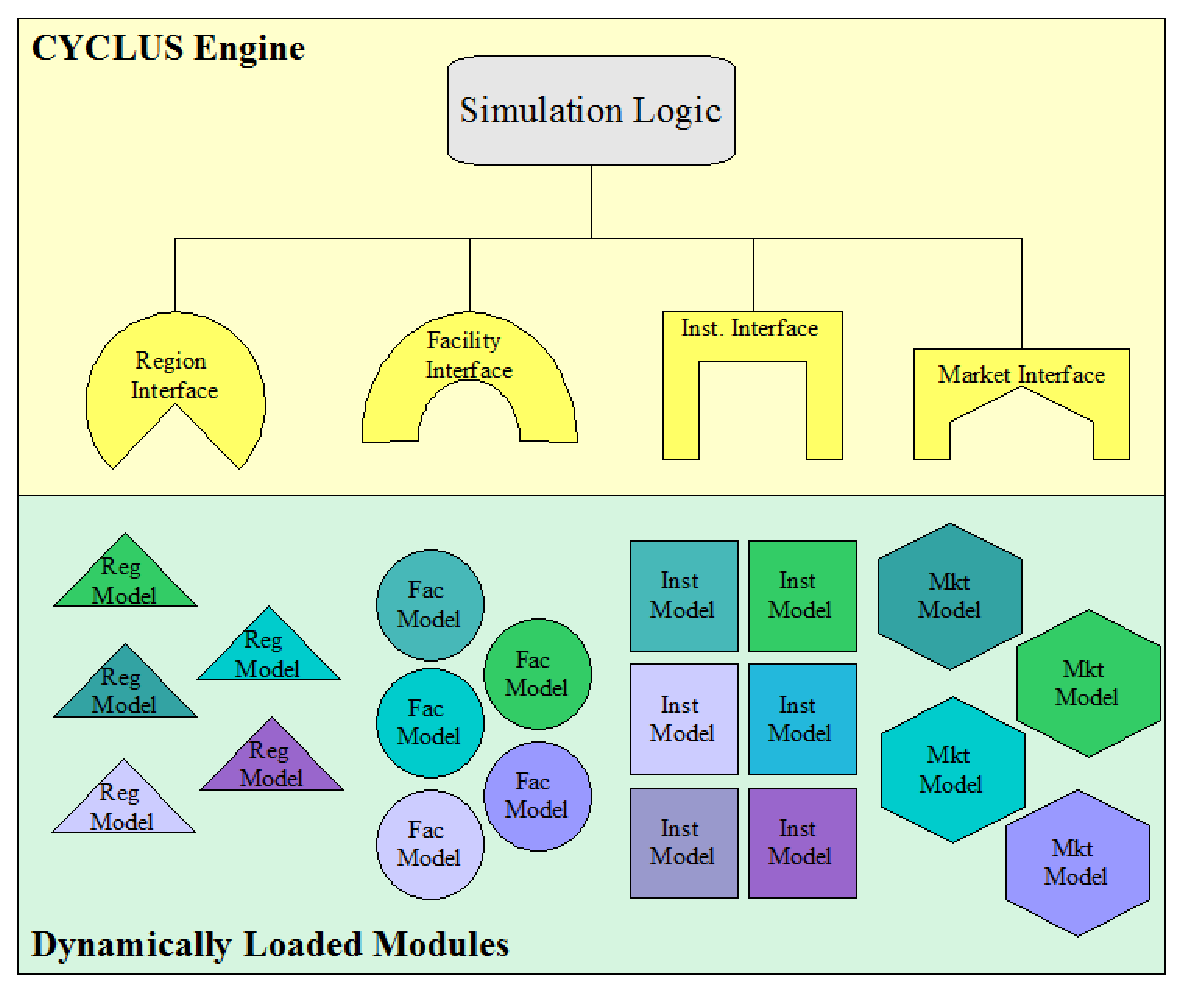
\includegraphics[height=5cm]{interfaces.eps}
    \end{center}
    \caption{Interface of Cyclus Models with the Engine} 
    \label{fig:interfaces}
  \end{figure}
\end{frame}
